
现在已经有了基准测试来测量读写内存的速度,看看如何访问内存中的数据,可以获得最佳性能。先从随机存取开始,读或写的每个值的位置都不可预测。

\subsubsubsection{4.4.1\hspace{0.2cm}随机访存的速度}

如果不多次运行基准测试,并对结果进行平均(基准库可以做到这一点),那么测量结果可能会相当混乱。在合理的运行时间(分钟)内,可能会看到如下结果:

%\hspace*{\fill} \\ %插入空行
\begin{center}
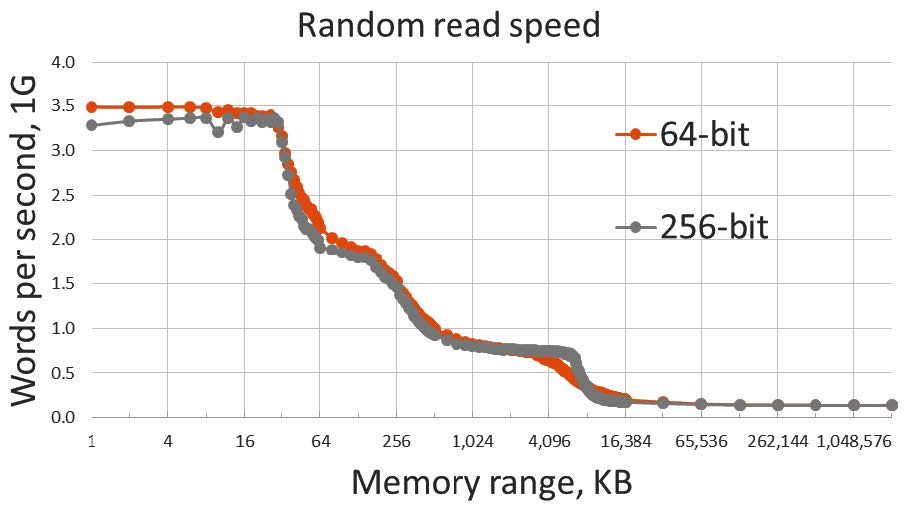
\includegraphics[width=0.9\textwidth]{content/1/chapter4/images/3.jpg}\\
图4.3 - 随机读取速度与内存大小的关系
\end{center}

图4.3中的基准测试结果显示,每秒从内存中读取的数据(以十亿为单位),长度为64位整数或265位整数(分别为\texttt{long}或\texttt{\_\_m256i})。同样的值也可以表示为,读取指定大小的单个整数所花费的时间:

%\hspace*{\fill} \\ %插入空行
\begin{center}
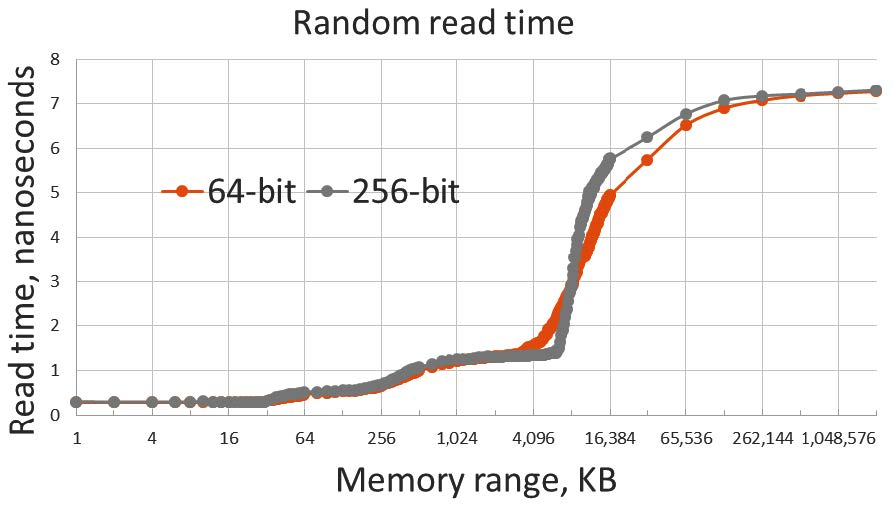
\includegraphics[width=0.9\textwidth]{content/1/chapter4/images/4.jpg}\\
图4.4 - 读取一个数组元素的时间与数组大小的关系
\end{center}

首先,没有单一的内存速度。在我所使用的计算机上,读取一个64位整数所需的时间从0.3纳秒到7纳秒不等。读取少量数据要比读取大量数据快得多。可以从这些图中看到缓存的大小,32KB的L1缓存速度很快,数据量都能装入L1缓存,读取速度就不依赖于数据量。超过32KB的数据,读取速度就开始下降。数据现在适合L2缓存,它更大(256KB),但速度更慢。数组越大,适合快速L1缓存的部分就越少,访问速度越慢。

如果数据从L2缓存溢出,读取时间会增加得更多,必须使用L3缓存。不过,L3缓存要大得多,所以直到数据大小超过8MB时才会发生变化。这时,才真正开始从主存读取数据。数据都是在第一次接触时从内存中移动到缓存中的,所有后续的读取操作都只使用缓存。如果需要一次访问超过8MB的数据,那么其中的一些数据必须从主内存中读取(不同的CPU模型的缓存大小不同)。当然,不要马上去除缓存的好处是,只要大多数数据适合于缓存,至少在某种程度上是有效的。当数据量超出缓存大小几倍,读取时间完全取决于从内存中检索数据所花费的时间。

在缓存中找到某个变量进行读或写,称之为\textbf{缓存命中}。如果没有找到,就注册一个缓存缺失事件。当然,L1缓存缺失可以是L2命中。一个L3缓存缺失意味着必须从主存加载数据。

从内存中读取一个整数需要7纳秒。按照处理器的标准,这是非常长的时间,CPU每纳秒可以做几个操作。还需要注意的是,CPU可以在从内存中读取一个整数值所花费的时间,可以执行大约50个算术运算,除非该值恰好已经在缓存中。很少有程序需要对每个值执行50个操作,这意味着CPU很可能没有得到充分利用,除非能够找到一些加速内存访问的方法。

最后,以每秒整数为单位的读取速度并不取决于整数的大小。从实用的角度来看,如果使用256位的指令来读取内存,可以读取4倍的数据。当然,SSE和AVX加载指令可以将值读入不同的寄存器,因此还可以使用SSE或AVX SIMD指令进行计算。更简单的情况是,只需要将大量数据从内存中的一个位置复制到另一个位置。测试表明,复制256位字比64位字快4倍。当然,现在有了库函数可以进行内存复制,比如:\texttt{memcpy()}或\texttt{std::memcpy()},并对其进行了优化,以获得最佳的效率。

速度不依赖于数据大小这一事实还有另一个暗示,读取速度受延迟影响,而不是带宽的限制。延迟是发出数据请求和检索数据之间的事件。带宽是内存总线在给定时间内可以传输的数据总量。从64位到256位在同一时间内传输的数据是64位的4倍。也就是,我们还没有达到带宽限制。这似乎是一个纯理论的结论,它确实对编写高效程序有重要的影响。

最后,我们可以测试写入内存的速度:

%\hspace*{\fill} \\ %插入空行
\begin{center}
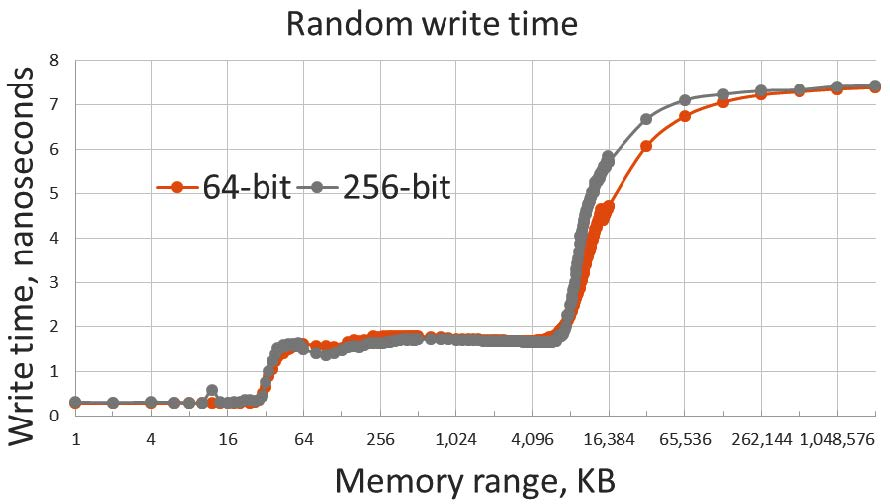
\includegraphics[width=0.9\textwidth]{content/1/chapter4/images/5.jpg}\\
图4.5 - 数组元素的写入时间与数组大小的关系
\end{center}

随机读写有非常相似的性能,但是这会因不同的硬件而不同。在前面观察到的读取内存的速度也适用于写入,在图4.5中看到了缓存大小的影响。如果涉及到主内存,则写入的总体等待时间会非常长,而且一次写入多个词会更有效率。

能否得出内存访问对性能影响的结论?一方面,如果需要重复访问少量的数据(小于32KB),就不必为此担心。当然,重复是这里的关键,无论计划访问多少内存,第一次访问的内存位置都必须接触主存(直到读取整个数组并返回开始,计算机才知道数组很小——第一次读取一个小数组的第一个元素看起来与读取第一个元素完全一样大数组的)。另一方面,如果必须访问大量的数据,那么内存速度可能会成为首先关心的问题:7纳秒/个的速度,能等得起吗?

有几种提高内存性能的技术,将会在本章中看到。我们也会研究如何改进我们的代码,先看看硬件。

\subsubsubsection{4.4.2\hspace{0.2cm}顺序访存的速度}

我们已经测试了在任意位置访问内存的速度,每一次内存访问实际上都是新的。我们正在读取的整个数组会加载到能够放入的最小缓存中,然后随机读写该缓存中的不同位置。该数组不适合缓存,然后随机访问内存中的不同位置,并且每次访问(对于我使用的硬件)都会产生7纳秒的延迟。

随机访存在程序中经常发生,但同样频繁的是顺序访存,从第一个元素到最后一个元素的顺序处理一个大数组。这里的随机和顺序访问是由存储器地址的顺序决定的,有可能出现误解的是,链表是不支持随机访问的数据结构(意味着不能直接跳到列表的中间),必须从头元素开始按顺序访问。如果每个链表元素在不同的时间分配,那么顺序遍历列表很可能是以随机顺序访问内存。另一方面,数组是一种随机访问数据结构(可以随时访问任何元素)。然而,从数组的开始读取到结束,顺序访问内存,按照单调递增的地址顺序。除非另有说明,在本章讨论顺序访问或随机访问时,只关心访问内存地址的顺序,而非数据结构。

顺序访存的性能也与随机方式不同。下面是顺序写入的结果:

%\hspace*{\fill} \\ %插入空行
\begin{center}
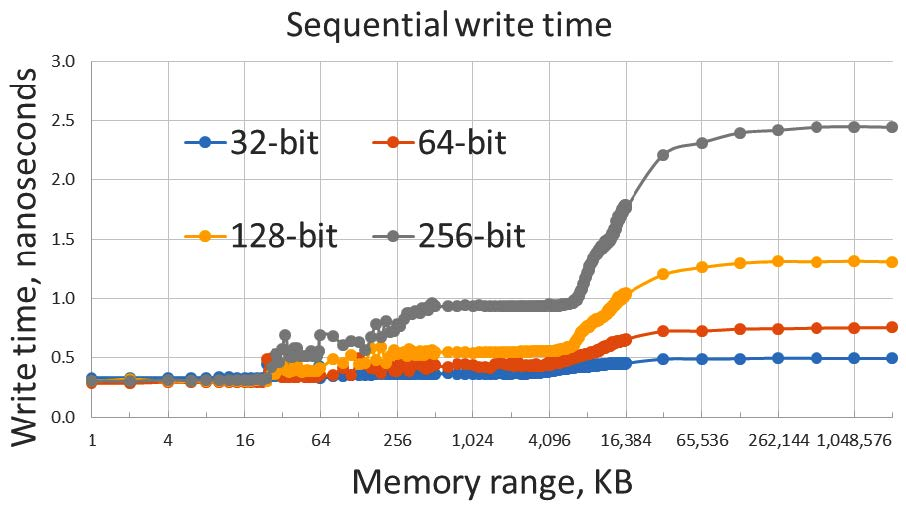
\includegraphics[width=0.8\textwidth]{content/1/chapter4/images/6.jpg}\\
图4.6 - 顺序访存,数组元素的写入时间与数组大小的关系
\end{center}

图的整体形状和以前一样,但不同之处和相似之处同样重要。首先,需要注意的是纵轴的刻度,时间值比我们在图4.5中看到的要小得多。写一个256位的值只需要2.5纳秒,而64位的整数只需要0.8纳秒。

第二个区别是数据块不同时,曲线不再相同。需要注意的是,此结果高度依赖硬件。许多系统中,将会看到与前一节中的结果更加相似的结果。在我使用的硬件上,对于不同大小的数据块,L1缓存的顺序写时间是相同的,但对于其他缓存和主存则不同。在主存写入时,可以观察到,写入64位整数的时间,并不是写入32位整数所需的时间的两倍,对于更大的数据,每次数据量加倍时,写入时间都加倍。这说明,限制不是每秒可以写多少个数据块,而是每秒可以写多少个字节:对于所有数据块的大小(除了最小的一个),每秒写入的字节数是相同的。现在限制速度的不是延迟,而是带宽。以总线能够传输的最快速度推送到内存中,无论将它们分为64位的数据块,还是256位的数据块,现在都已经达到了内存的带宽限制。本章中,这个结果比之前所做的观察更加依赖硬件。在许多机器上,会出现内存足够快,而CPU无法饱和使用其带宽的情况。

虽然与缓存大小相对应的曲线中的“阶梯”仍然可见,但不那么明显,也不那么陡峭。现在已经有了结果,也进行了观察。那结论是什么呢?

\subsubsubsection{4.4.3\hspace{0.2cm}硬件中的内存性能优化}

三个观察结果需要结合起来,可以看出硬件使用了某种隐藏延迟的技术(除了改变内存访问顺序外,没有做任何事情来提高代码的性能,所以这些改进都归功于硬件)。当随机访问主内存时,每次访问在我的机器上需要7纳秒。这是从特定地址的数据请求到交付至CPU寄存器所花费的时间,这个完全由访存延迟决定(不管请求了多少字节,必须等待7纳秒)。当按顺序访问内存时,硬件可以开始传输数组的下一个元素。访问第一个元素仍然需要7纳秒,顺序访问内存时,硬件可以马上访问数组的下一个元素。第一个元素仍然需要7纳秒来访问,此后硬件以CPU和内存总线处理它的速度将整个数组从内存中写入或读出。数组中第二个和之后元素的传输,有可能在CPU发出数据请求之前就开始了。因此,延迟不再是限制因素,而带宽才是。

当然,这是假设硬件已知要按顺序访问整个数组,以及这个数组有足够大。在现实中,硬件什么都不知道,就像上一章学习的条件指令一样,内存系统中有学习回路,可以做出有根据的猜测。在我们的示例中,出现了\textbf{预取}。当内存控制器注意到CPU已经连续访问了几个地址,就会假设这个地址会继续使用,并为访问下一个内存位置做准备,将数据传输到L1缓存中(用于读操作),或者在L1缓存中腾出空间(用于写操作)。理想情况下,预取技术允许CPU始终以L1缓存的速度访问内存,当CPU需要每个数组元素时,其已经在L1缓存中了。实际情况是否符合这种理想情况,要取决于CPU在访问相邻元素之间做了多少工作。在基准测试中,CPU几乎不做任何工作,而预取则落后了。期望线性顺序访问,则没有办法足够快地在主内存和L1缓存之间传输数据。然而,预取在隐藏内存访问延迟方面非常有效。

预取并不是基于如何访问内存的预测或先验(有一些特定于平台的系统调用,允许程序通知硬件某个范围的内存将被顺序访问,但这是不可移植的,而且在实践中很少奏效)。相反,预取尝试在访问内存时检测访存模式。因此,预取的有效性取决于,访存模式和下一次访问的位置。

关于预取模式检测的局限性有很多信息,其中很多都已经过时。在较早的文献中,可以读到按向前顺序访问内存(对于数组\texttt{a},从\texttt{a[0]}到\texttt{a[N-1]})比向后访问更高效。这对现代CPU来说都不再适用,而且现在已经不是这样了。如果我开始准确地描述,哪些模式在预取方面是有效的,哪些模式是无效的,那么该书就有落入同样陷阱的风险。最后,如果算法需要特定的内存访问模式,并且想知道预取能否处理它,最可靠的方法是使用与随机内存访问类似的基准测试进行测试。

通常,预取对于访问内存的递增顺序和递减顺序都有效。在预取调整到新的模式之前,反转方向会有一些性能损失。像访问数组中的每4个元素这样的跨步处理,会被检测和预测,其效率与密集的顺序访问一样。预取能够检测多个并发跨步(即访问每3个和每7个元素),但当硬件功能从一个处理器转移到另一个处理器时,必须自己对数据进行紧致化处理。

硬件非常成功地采用的另一种性能优化技术:\textbf{流水线}或\textbf{硬件循环展开}。在上一章中我们已经了解过,这种技术可以用来隐藏由条件指令引起的延迟。通常,流水线也可用于隐藏内存访问的延迟。看一下这个循环:

\begin{lstlisting}[style=styleCXX]
for (size_t i = 0; i < N; ++i) {
	b[i] = func(a[i]);
}
\end{lstlisting}

每次迭代从数组中读取一个值\texttt{a[i]},进行一些计算,并将结果存储在另一个数组\texttt{b[i]}中。读和写都需要时间,可以期望循环执行的时间轴是这样的:

%\hspace*{\fill} \\ %插入空行
\begin{center}
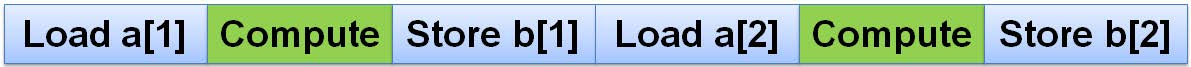
\includegraphics[width=0.9\textwidth]{content/1/chapter4/images/7.jpg}\\
图4.7 - 非流水线循环的时间线
\end{center}

这个操作序列会让CPU在大部分时间里等待内存操作完成。硬件将提前读入指令流,并覆盖彼此不依赖的指令序列:

%\hspace*{\fill} \\ %插入空行
\begin{center}
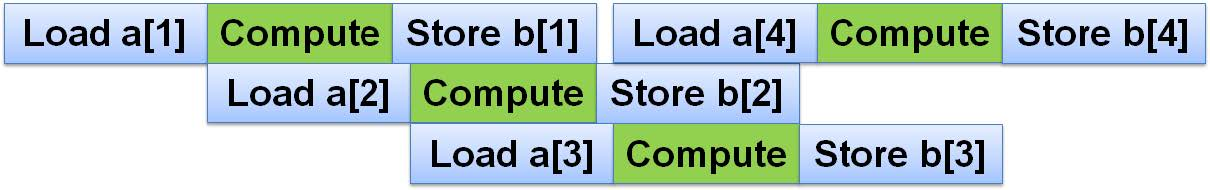
\includegraphics[width=0.9\textwidth]{content/1/chapter4/images/8.jpg}\\
图4.8 - 流水线(展开)循环的时间线
\end{center}

假设有足够的寄存器,第二数组元素的加载可以在第一个数组元素读取后立即开始。简单来说,假设CPU不能一次加载两个值(大多数真正的CPU可以同时做多个内存访问,这意味着流水线可以更宽),当有输入值可用,第二组计算就开始。前几个步骤中,指令载入流水,CPU花费了大部分时间进行计算(如果来自不同迭代的计算步骤重叠,CPU甚至可以一次执行多个迭代,只要有足够多的计算单元)。

流水线可以隐藏内存访问的延迟,但这是有限制的。读取一个值需要7纳秒,需要读取一百万个值,最多需要7毫秒,这是无法避免的(假设CPU一次只能读取一个值)。流水线操作可以通过将计算与内存操作重叠来减少读取时间,在理想情况下,所有计算都在这7毫秒内完成。预取可以在我们需要它之前读取下一个值,从而减少读取时间,但前提是猜测正确。无论哪种方式,本章中所做的测量都展示了以不同方式访问内存的最佳情况。

测量内存速度和呈现结果方面,我们已经了解了基础知识,并了解了内存系统的通用属性。更详细或具体的测量方法留给读者作为练习,可以收集所需的数据,以便对特定应用程序的性能要求做出明智的决策。现在我们把注意力转到下一个阶段:知道内存是如何工作的,了解了可以在内存方面得到什么性能,那我们需要做些什么才能提高程序的性能呢?
















